%\documentclass[a4paper,11pt]{book}
\documentclass[a4paper,12pt,one side]{report}%book}
%\input{setbmp}
\usepackage{epsfig}
\usepackage{longtable}
\usepackage{enumerate}
%\usepackage{caption2}
\usepackage{afterpage}
\usepackage{graphicx}
\usepackage{multirow}
\usepackage{amsmath, amsfonts} 
\usepackage[left=3.5cm,top=1.5cm,right=3cm,bottom=4cm]{geometry}
\usepackage{setspace}           %%%%%%%%%%THIS IS for BOOK size
%\usepackage{lscape}
\usepackage{booktabs} % Allows the use of \toprule, \midrule and \bottomrule in tables
%\usepackage{parskip} 
  \hyphenpenalty=5000
  \tolerance=1000
%\oddsidemargin 1.48cm
%\evensidemargin .5cm
%\textwidth 17cm 
% Graphics files are in the figures/ directory
%\graphicspath{{figures/}}

\usepackage{lscape} % for landscape tables
%\usepackage{appendix}
\usepackage{cite}
\renewcommand{\baselinestretch}{1.7} %%%%%%% JSS added for line spaceing
%\input{style}   %************************ i have removed jss

%\pagestyle{bfheadings}
\begin{document}

\thispagestyle{empty}

\oddsidemargin 1.48cm
\evensidemargin .5cm
\begin{center}

{\Large \bf DESIGN AND FABRICATION OF THREE FINGERED GRIPPER : SIMULATION AND CONTROL USING ROS \\}

\vspace*{0.65cm}
{\large \textbf {Mini Project Report}}\\
{\normalsize \it Submitted in partial fulfillment of the award of the degree of M.Tech in\\  Robotics and Automation\\ of the APJ Abdul Kalam Technological University
}
%{\normalsize \it Registration Seminar Report}

%\vspace*{1cm}

%{\em M.Tech.}\\
%\vspace*{1.5mm}
%in\\
%\vspace*{1.5mm} 
%CET Centre for Interdisciplinary Research\\
%\vspace*{1.5mm} 
%(ROBOTICS AND AUTOMATION)\\
%\vspace*{.5cm}

%by


\vspace*{.5cm}

{\bf GOKUL SOMAN\\
{\bf Register No: TVE19ECRA08}
\vspace*{0.75cm}

%{\bf Prof: D. Das}
\vspace*{.5cm}

{\bf Second Semester}\\
{\bf Master of Technology}
\vspace*{0.75cm}
%\vspace*{1cm}


\begin{figure}[hbt]
%\centerbmp{1.2in}{1.4in}{iitlogo.bmp}
\centering
\centerline{
\includegraphics[scale=1]{ccc/cet_emblem.pdf}}
\end{figure}
\vspace*{0.75cm}


{\footnotesize CET CENTRE FOR INTERDISCIPLINARY RESEARCH}\\
{\small \bf COLLEGE OF ENGINEERING TRIVANDRUM}\\
{\small \bf KERALA\\
2020}
\end{center}
%\newpage
%\input{dedicate}
        %\newpage
       %\input{preface}
\newpage
\pagenumbering{roman}
%\chapter*{Certificate}
%\addcontentsline{toc}{chapter}{Certificate}
\thispagestyle{empty}

\vspace*{-0.3cm}
\begin{center}  {\large \bf CET CENTRE FOR INTERDISCIPLINARY RESEARCH}\vspace{0.1cm}\end{center}
\begin{center}  {\LARGE \bf COLLEGE OF ENGINEERING TRIVANDRUM}\vspace{0.1cm}\end{center}
\begin{center}  {\large \bf THIRUVANANTHAPURAM - 17}\vspace{0.1cm}\end{center}

\begin{figure}[hbt]
%\centerbmp{1.2in}{1.4in}{iitlogo.bmp}
\centering
\centerline{
\includegraphics[scale=0.6]{ccc/cet_emblem.pdf}}
\end{figure}


\begin{center}  {\Large \textit {Certificate}}\vspace{.1cm}\end{center}

\textit {   This is to certify that this report entitled \textbf{"DESIGN AND FABRICATION OF THREE FINGERED GRIPPER : SIMULATION AND CONTROL USING ROS"} is a bonafide record of the miniproject by  \textbf{Mr. Gokul Soman, Reg. No: TVE19ECRA08} and of Second Semester, M.Tech under our guidance towards the partial fulfillment of the requirements for the award of \textbf{M.Tech in Robotics and Automation} of the \textbf{APJ Abdul Kalam Technological University }during the year 2020.}

\begin{singlespace}
\begin{center}
\begin{tabular}{ p{6cm} p{2cm} p{6cm} }
Guided By:& &Head Of Department:\\
\vspace{0.02cm}\textbf{Prof. Ajith R R }& &\vspace{0.02cm}\textbf{Dr. Sindhu G} \\ 
Asst. Professor& &Dean (Research) \\
Dept. of Mechanical Engg. & &College of Engineering,\\
College of Engineering, Tvm & &Trivandrum \\ 
\end{tabular}
\end{center}
\vspace{0.1cm}
\begin{center}
Mini Project Co-ordinators\\\vspace{0.1cm}
\begin{tabular}{ p{6cm} p{2cm} p{6cm} } 
\textbf{Dr. Ranjith S Kumar}&&\textbf{Prof. Lalu V} \\ 
Asst. Professor&&Asst. Professor\\ 
Dept. of Mechanical Engg.&&Dept. of Electronics Engg.\\ 
College of Engineering, Tvm && College of Engineering,Tvm\\
\end{tabular}
\end{center}

\end{singlespace}
\newpage
%\input{acknow}
%\newpage
%\input{abstract}
%\addcontentsline{toc}{chapter}{Certificate}
\thispagestyle{empty}

\vspace*{1cm}
\begin{center}  {\Large \bf ABSTRACT}\end{center}
%%\begin{abstract}\vspace{1cm}
\noindent       The objective of this project is to design and develop a three fingered gripper with 8 DOF that can reconfigure itself  to grasp different targets. It is an underactuated system with 3 articulated fingers driven by four motors. Each finger can be grasped with two degrees of freedom by a single motor, one of which is fixed to the frame, and the other two fingers can also rotate in the opposite direction with two degrees of freedom along the palm surface. Grasping action of each finger is independently controlled by a motor. The symmetrically opposable fingers centered on parallel joint axes can be rotated from 0 to 180° by the fourth motor. 

The prototype could be used as an end effector of ABB IRB 120 in Robotics lab. Underactuated hands could be used in many situations for its lightweight and flexible features for applications in medical, aerospace and unmanned systems.

The procedure includes different stages like specification definition, mechanical design, torque computation for motor selection, simulation, developing the control system and prototype testing. These stages cover various aspects like stress analysis, forward and inverse kinematics, and dynamic modelling. Finally, the developed prototype will be tested to see if it meets the specification definition.



\newpage
%\input{acknow}
%\newpage
%\input{abstract}
%\addcontentsline{toc}{chapter}{Certificate}
\thispagestyle{empty}

\vspace*{1cm}
\begin{center}  {\Large \bf Acknowledgment}\end{center}
%%\begin{abstract}\vspace{1cm}
\par
I have great pleasure in expressing my gratitude and obligations to  \textbf{Prof. Jaimon Cletus}, Guide, Department of Mechanical Engineering, College of Engineering, Trivandrum  for his valuable guidance and suggestions to make this work a great success.

I express my thanks to  \textbf{Dr. Ranjith S Kumar}, Asst. Professor Department of Mechanical Engineering, College of Engineering, Trivandrum for all the guidance and encouragement  in the fulfillment of this work.

I express my gratitude to \textbf{Prof. Lalu V}, Asst. Professor Department of Electronics Engineering, College of Engineering, Trivandrum, for all  necessary help extended to me in the fulfillment of this work.

I express my gratitude to \textbf {Dr. Jisha V R}, Asst. Professor , Department of Electrical Engineering, College of Engineering, Trivandrum for all the support extended to me in the fulfillment of this work.

\par


I also acknowledge my gratitude to other members of faculty in the Department of Electrical Engineering ,Mechanical Engineering, Electronics Engineering, staffs of FAB lab, staffs of machine shop, staffs of CET school of management, my family and friends for their whole hearted cooperation and encouragement. Above all, I thank GOD Almighty, without whose help, I wouldn't have reached this far.

 \newpage
\tableofcontents 	\cleardoublepage%\newpage 
\addcontentsline{toc}{chapter}{List of Figures} 
\listoffigures 	\cleardoublepage %\newpage 

\addcontentsline{toc}{chapter}{List of Tables}
\listoftables 	\cleardoublepage%\newpage
%\input{los1} \newpage
%\input{losjss} \newpage   %%%LIST OF SYMBOLS
\pagenumbering{arabic}

%*************************************************************************************************
\chapter{Introduction}
\label{chapintro}
\section{Three Fingered Gripper}
The robot end effector is the bridge between the robot arm and the environment around it. The actions of the gripper vary with the tasks. A large variety of gripper designs mostly two fingered can be seen in industries performing assembly tasks. An object with circular cross-section cannot be held properly with these set of two fingers atleast not without indeterminacy of position. Since circular and rectangular objects partly or wholly characterize the vast majority of parts encountered in industry in general, a "universal" robot gripper must be able to handle these effectively.

\par From an anthropomorphic point of view, Schlesinger has defined the six basic prehensile patterns of the human hand. Their mechanical equivalents require a minimum of three fingers. Therefore, three fingers seem to be essential for the manipulation of objects in general.

\par include pic of prehensile patterns
\par The mechanical equivalents of basic prehensile patterns:
(a) Two-finger, b) three-finger concentric, and c) three-
finger wrap. These three modes allow grasping of most objects
commonly found in assembly operations.

		
\section{Underactuation}
\par Underactuated robotic hands are the intermediate solution between robotic hands for manipulation , which have the advantages of being versatile, guarantee a stable grasp, but they are expensive, complex to control and with many actuators; and robotic grippers, whose advantages are simplified control, few actuators, but they have the drawbacks of being task specific, and perform an unstable grasp. 

\par An underactuated mechanism allows the grasping of objects in a more natural and more similar to the movement obtained by the human hand. \cite{Martinoli2012SpringerPreface}


%\begin{figure}[htbp]
		%	\begin{center}
		%		\includegraphics[width=0.5\textwidth, angle=0]{img/rrp.jpg}
		%		\caption{ Spherical Robot Configuration}
		%	\end{center}
	%	\end{figure}
		
		
\section{Objectives}
\label{Objectives} 
The project deals with design, simulation and fabrication of a three fingered gripper . The primary objectives of this project are:-\
\begin{itemize}
\item Design a 3 fingered gripper for a basic pick and place application.
\item Perform simulation of the gripper in ROS platform
\item Fabricate the gripper and perform a basic pick and place operation (attached to ABB IR 120) using ROS as the trajectory planner.
\end{itemize}

\section{Outline of the Report}

This project report is organised as follows: 
\par 
Chapter 1 presents background of the work that describes the way through which the paper is modified into the main objective. 
\par
Chapter 2 deals with the literature review. A brief survey of the previous research works of the topic has been discussed in this section.
\par
Chapter 3 deals with the methodology of the work and specifications of the robot under which it is built and finally a brief description about the whole system is mentioned.
\par
Chapter 4 deals with the simulation part which includes the creation of URDF file, simulation robot in Gazebo and finally interfacing the actual hardware with ROS.
\par
Chapter 5 deals with the Fabrication and Hardware Description in detail.
\par
Chapter 6 discuss about the ROS Control of Hardware.
\par
Chapter 7 deals with Simulation Results.
\par
Chapter 8 presents the project conclusion.
\par
Chapter 9 is the list of research papers that were referred for this project.
%...................................................................................%


\chapter{Literature Review}


%-----------------------------------------------------------------

\chapter{Mechanical Design and Modelling}
\section{Methodology}
The methodology adopted for is discussed here. It is a simple and systematic approach. The entire work can be split in to two sections as described.
\subsubsection{Simulation Phase}
\begin{itemize}
    \item Create CAD model for simulation satisfying the specifications.
    \item Create Moveit! package and define controllers.
    \item Perform Real time simulation in Gazebo using Moveit! Rviz motion planning.
\end{itemize}

\subsubsection{Fabrication Phase}
\begin{itemize}
    \item  Compute the maximum torque requirement at each joints and select joint motors accordingly.
    \item Create CAD model for actual fabrication.
    \item Fabricate the robot and demonstrate real time control on actual robot.
\end{itemize}

\section{Robot Specifications}


%\section{Work Envelope}


\section{System Description}

 The development of the robot also includes two phases simulation phase and fabrication phase. Simulation phase includes creating CAD model for simulation satisfying the specifications, Moveit package and define controllers. Finally performing real time simulation in Gazebo using Moveit-Rviz motion planning. Fabrication phase includes computation of the maximum torque requirement at each joints and selection of joint motors accordingly. Creating CAD model for actual fabrication. After fabrication of the robot, demonstration of real time control on actual robot. The block diagram representation of the desired configuration is shown.
 
 \begin{figure}[h]
    \centering
    \includegraphics[scale=0.7]{img/systemdescrip.png}
    \caption{Block diagram of RRP configured robot}
    \label{fig:systemdescrip}
\end{figure}
 



%\chapter{Mathematical Modelling and Torque Computation}
    
 %----------------------------------------------------------%


\chapter{Simulation Using ROS}
\par ROS, the Robot Operating System, is an open source framework for writing robot
software and for getting robots to do things. ROS is meant to serve as a common
software platform for people who are building and using robots. ROS follows the
Unix philosophy of software development in several key aspects. ROS systems
are comprised of a large number of independent programs that are constantly
communicating with each other. This paradigm was chosen to encourage the reuse
of robotics software outside the particular robot and environment that drove its
creation.

\par Roscore is a service that provides connection information to nodes so that they
can transmit messages to one another. The most common way to do that is
through topics. A topic is a name for a stream of messages with a defined
type. Every node connects to roscore at startup to register details of the message
streams it publishes and the streams to which it wishes to subscribe. ROS graph
node represents a software module that is sending or receiving messages.Every
ROS system needs a running roscore ,since without it, nodes cannot find other
nodes. Catkin is the ROS build system: the set of tools that ROS uses to
generate executable programs, libraries, scripts, and interfaces that other code
can use.Before you start writing any ROS code, you need to set up a workspace for this code to live in. A workspace is simply a set of directories in which a
related set of ROS code lives. ROS software is organized into packages, each of
which contains some combination of code, data, and documentation. The ROS
ecosystem includes thousands of publicly available packages in open repositories,
and many thousands more packages are certainly lurking behind organizational
firewalls.
\par First step of simulation using ROS is the modelling of the SCARA robot from the
URDF file generated by the solid modelling and computer aided design (CAD)
software Solidworks.

\section{Modelling The Robot URDF}

In ROS robot models are represented in an XML format called Unified Robot Description Format (URDF). This format is designed to represent a wide variety of robots from a two-wheeled toy to a walking humanoid. URDF is similar to the Simulation Description Format (SDF), which is commonly used to build Gazebo environments around existing robots. URDF is only capable of representing robots whose kinematics can be described by a tree.
\newline
On startup, the URDF model of the robot was loaded into the parameter server, under the standard name robot description.
The joint state publisher , in response to the slider state in the GUI, is publishing sensor msgs -Joint State messages on the joint states topic. Each message declares the position of each joint in the system. Another node, the robot state publisher, reads the URDF model from the parameter server and is subscribed to joint states . This node combines the 1D position of each joint with the kinematic model to calculate a tree of 6D (position and orientation) coordinate transforms that describe where in space the robot’s links are with respect to each other (in other words, it performs forward kinematics).
\newline
The robot state publisher is commonly used with robots (both real and simulated) to handle the common task of forward kinematics, allowing the authors of robot drivers to publish just the individual joint state information and not the full coordinate transform tree. And as Rviz
is used extensively in ROS development, especially for visualization of data related to coordinate transforms, the URDF display tool is really just a combination of commonly used ROS tools with a simple front end GUI that allows to  supply fake
joint position information.
\newline
URDF format folder is needed for visualizing in Rviz ,simulation in Gazebo and hardware ROS control. To export URDF from Solidworks we need to do the following steps.
\newline
Before exporting to URDF file, change to reference pose of the robot. The first joint is revolute from 0 radians to 6.28 radians. So the joint should be keept in 0 radian angle for best response when interfacing with hardware. Negative values can be used in Rviz and Gazebo Simulation. But when interfacing with Arduino for hardware implementation of negative values are not expected. 
The second joint is revolute joint, the limit angle minimum is 0 radian and maximum is 2.8 radian(160 degree). 
The third joint is prismatic joint, according to this case keeping the prismatic joint in retracted position is expected to give a radial traverse of 200mm (for the prismatic joint. \newline
Step 1 : Click file. A drop down list will appear. Click on Export as URDF option. \newline
Step 2 : A dialog box will appear probably on left side of the window. \newline
Step 3 : Give name of base link. Give base\_link as fixed joint. The origin reference axis will be automatically generated if we give appropriate option. Select the links we are considering as fix. In this case base links are fixed.\newline
Step 4 : In the cell for entering number of child links, give 1(in this case). A child link will be created.\newline
Step 5: Double click on the child link . Replace the name empty link by giving the name as link1(in this case). Give joint name as R1 (in the case. R1 denotes Revolute Joint 1).  Select Joint type as revolute joint.\newline
\begin{figure}
    \centering
    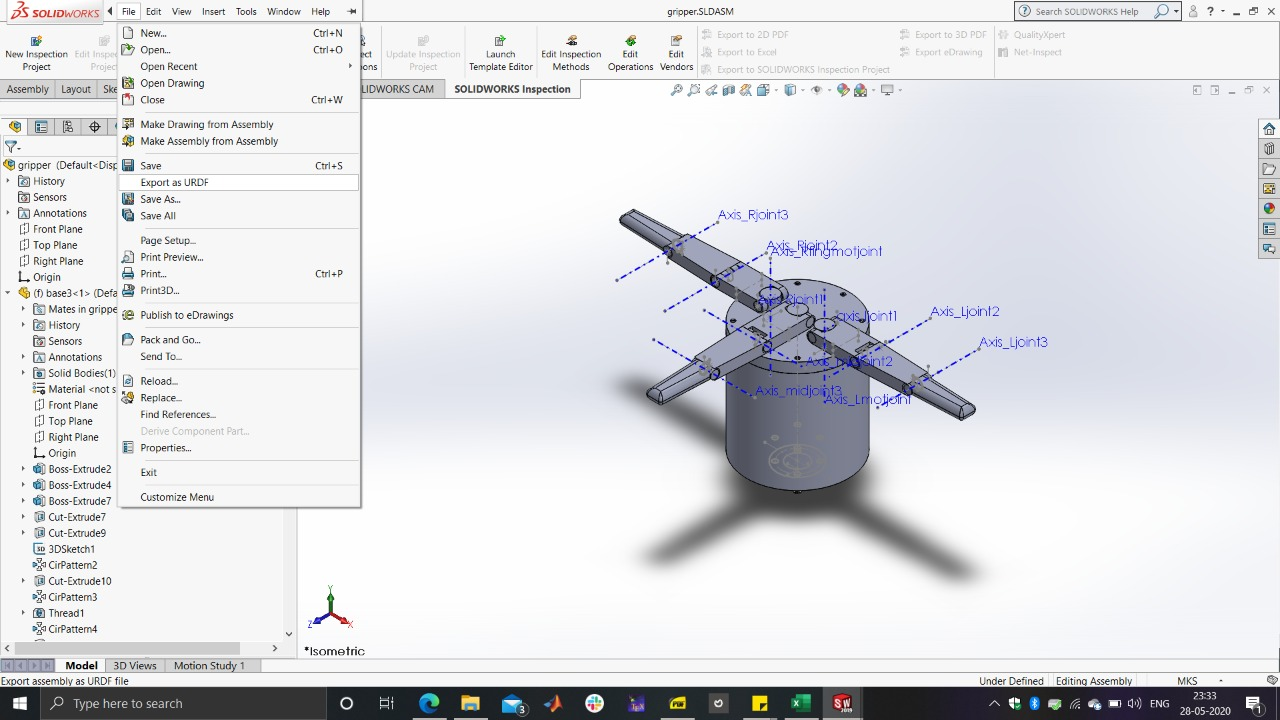
\includegraphics[scale=0.3]{gripper_images/Create_URDF.jpeg}
    \caption{Creating URDF using URDF plugin in Solidworks}
    \label{fig:my_label}
\end{figure}
Step 6 : In the cell for entering number of child links, give 1(in this case). A child link will be created.\newline
Step 7: Double click on the child link . Replace the name empty link by giving the name as link2(in this case). Give joint name as P2(in the case. P2 denotes Prismatic Joint 2). Select joint type as prismatic joint.\newline
Step 8 : In the cell for entering number of child links, give 1(in this case). A child link will be created.\newline
Step 9: Double click on the child link . Replace the name empty link by giving the name as link3(in this case). Give joint name as R3(in the case. R3 denotes Revolute Joint 3). Select joint type as reolute joint. \newline
Step 10: A window will be opened. Click on first joint name R1. Change the joint angles minimum and maximum values to 0 and 6.24 radians respectively. Give effort value as 100 and velocity as 1.\newline
Step 11: Double Click on second joint name P2. Change the joint distance minimum and maximum values to 0 and 0.17 metres respectively.  Give effort value as 100 and velocity as 1.\newline
Step 12: Double Click on third joint name R3. Change the joint angles minimum and maximum values to 0 and  3.14 radians respectively.  Give effort value as 100 and velocity as 1.\newline
Step 13: Click on Finish. \newline

The URDF folder will be created in the destination given. Copy the folder to some location in drives so that we can access from Windows. URDF is an XML format for representing a robot model.


\section{Generating Move-It Package }

    \subsection{Steps for generating moveit! package}
   \begin{itemize}
    \item Intialising the move it package by \textbf{roslaunch moveit\_setup\_assistant setup\_assistant.launch}.
    \item A new moveit package window is opened, click on \textbf{create New Moveit! Configuration Package }$\rightarrow$ Browse then from the desired location the package robot\_1 is selected from which URDF is loaded on the  moveit package. 
    \item If the robot model is successfully loaded, robot model appears on  window next.
\item  Next\textbf{ Self-Collision matrix} needs to be generated. It checks for each link pair and categorizes the links as always in collision, never in collision, default in collision, adjacent links disabled, and sometimes in collision, and it disables the pair of links which makes any kind of collision.
\item \textbf{Virtual Joint} is for mobile robots and hence is not needed here.
\item  \textbf{Planning group} is a group of joints/links in a robotic arm  which plans together in order to achieve a goal position of a link or the end effector.Two planning groups are to be created, one for the arm and one for the gripper,since end-effector is not used, only one planning group is created.
\end{itemize}
\begin{figure}
    \centering
    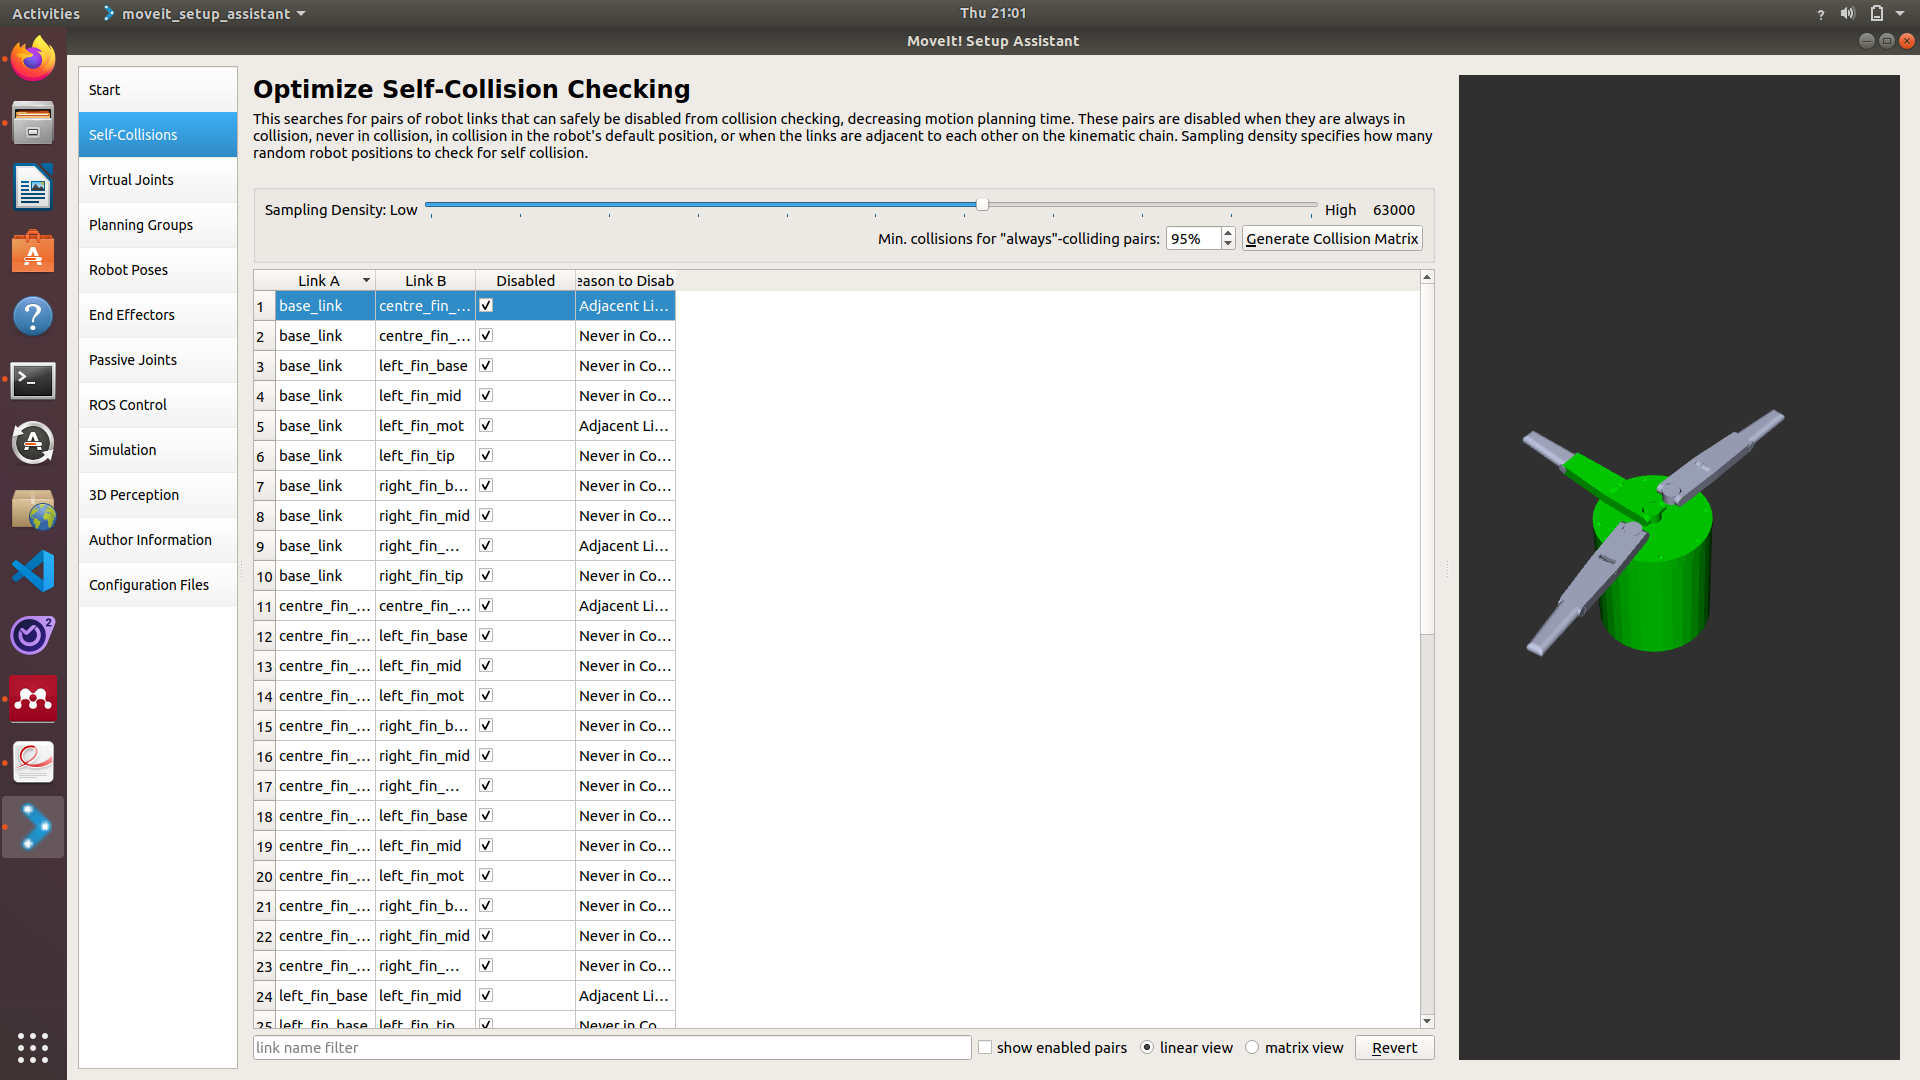
\includegraphics[scale=0.2]{gripper_images/setup_asst_startup.png}
    \caption{Moveit Setup Assistant startup}
    \label{fig:my_label}
\end{figure}
\begin{itemize}


\begin{figure}
    \centering
    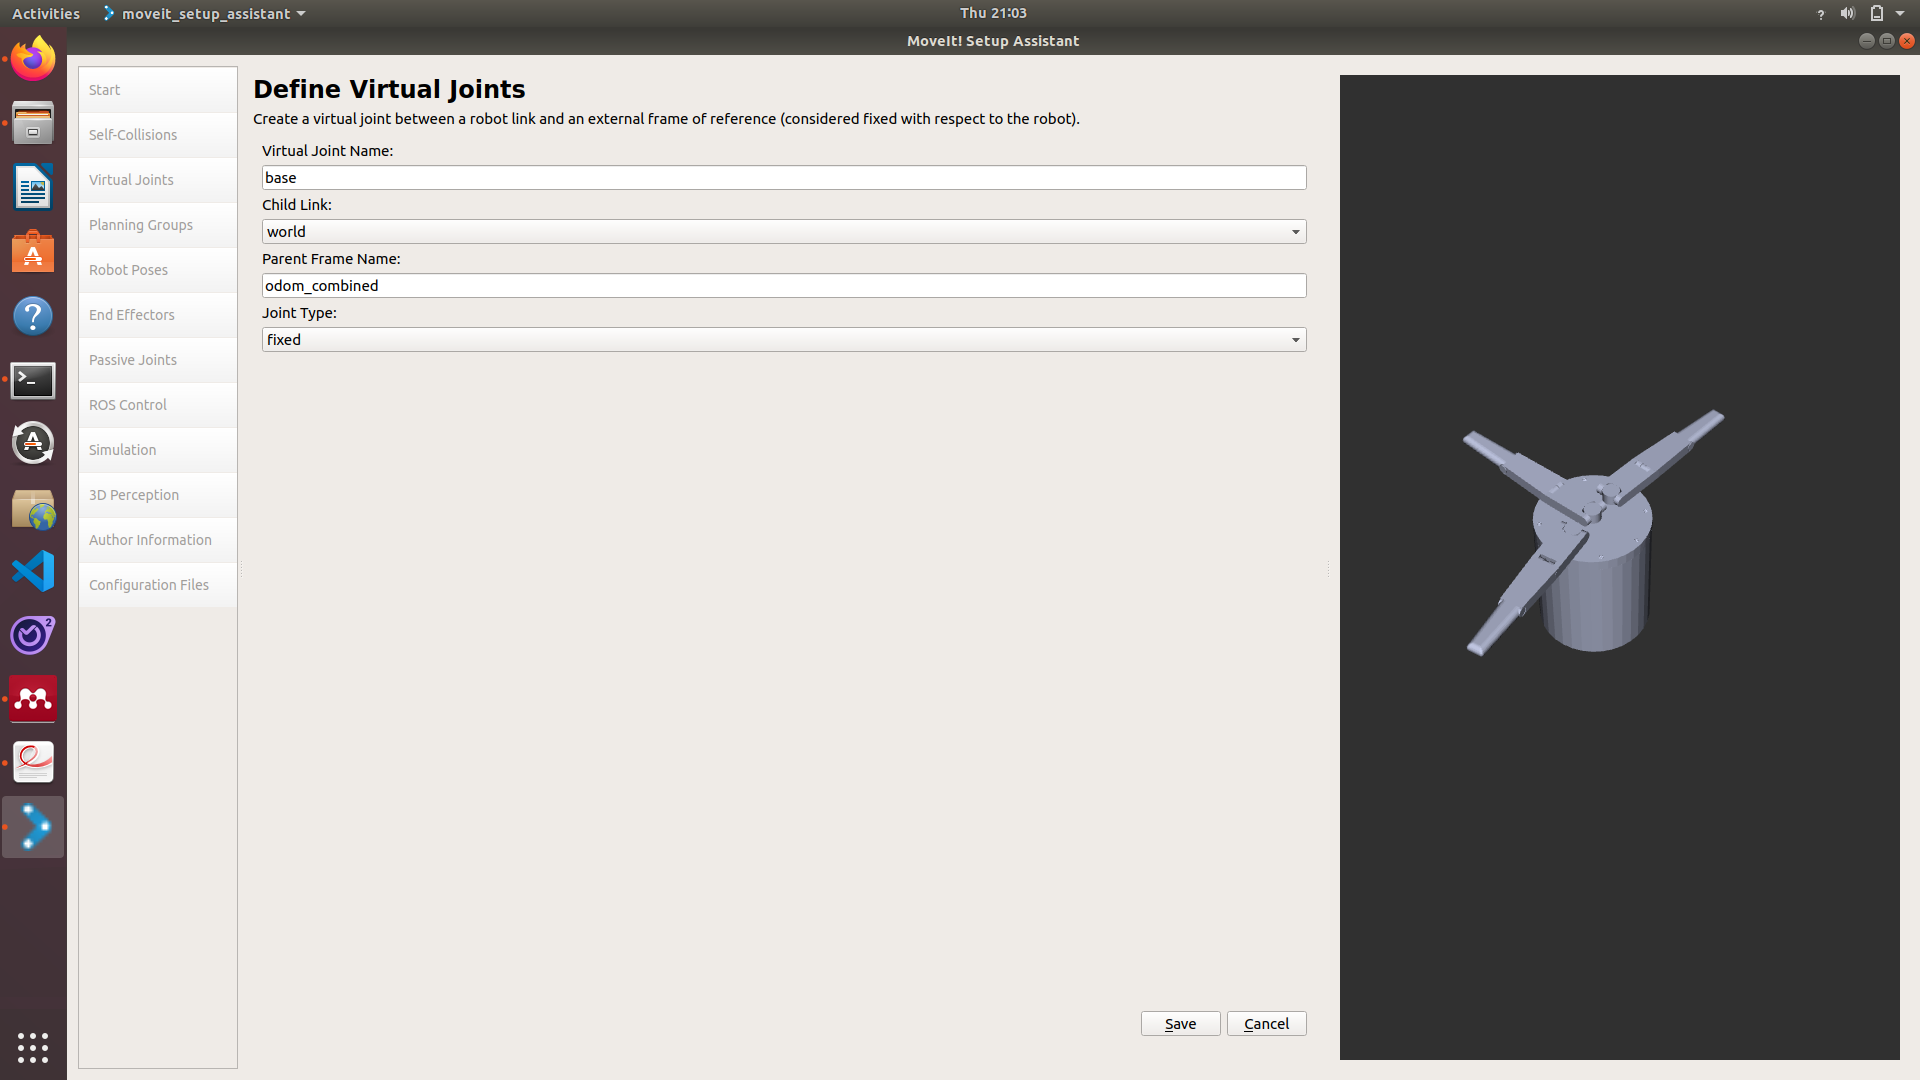
\includegraphics[scale=0.2]{gripper_images/Virtual_joints.png}
    \caption{Defining Virtual Joints}
    \label{fig:my_label}
\end{figure}

\item Select\textbf{ Planning Group}, planning group window appears, in this window  \textbf{Group Name} is given. Next is the selection of the \textbf{Kinematic Solver}. From the drop down box select \textbf{kdl\_kinematics\_plugin/KDL Kinematics Plugin}.
\item Then inside the \textbf{gripper group} ,\textbf{Kinematic 
Chain} is added, there \textbf{centre\_fin\_mid\_joint} to \textbf{right\_fin\_tip\_joint} have to be added. \begin{figure}
    \centering
    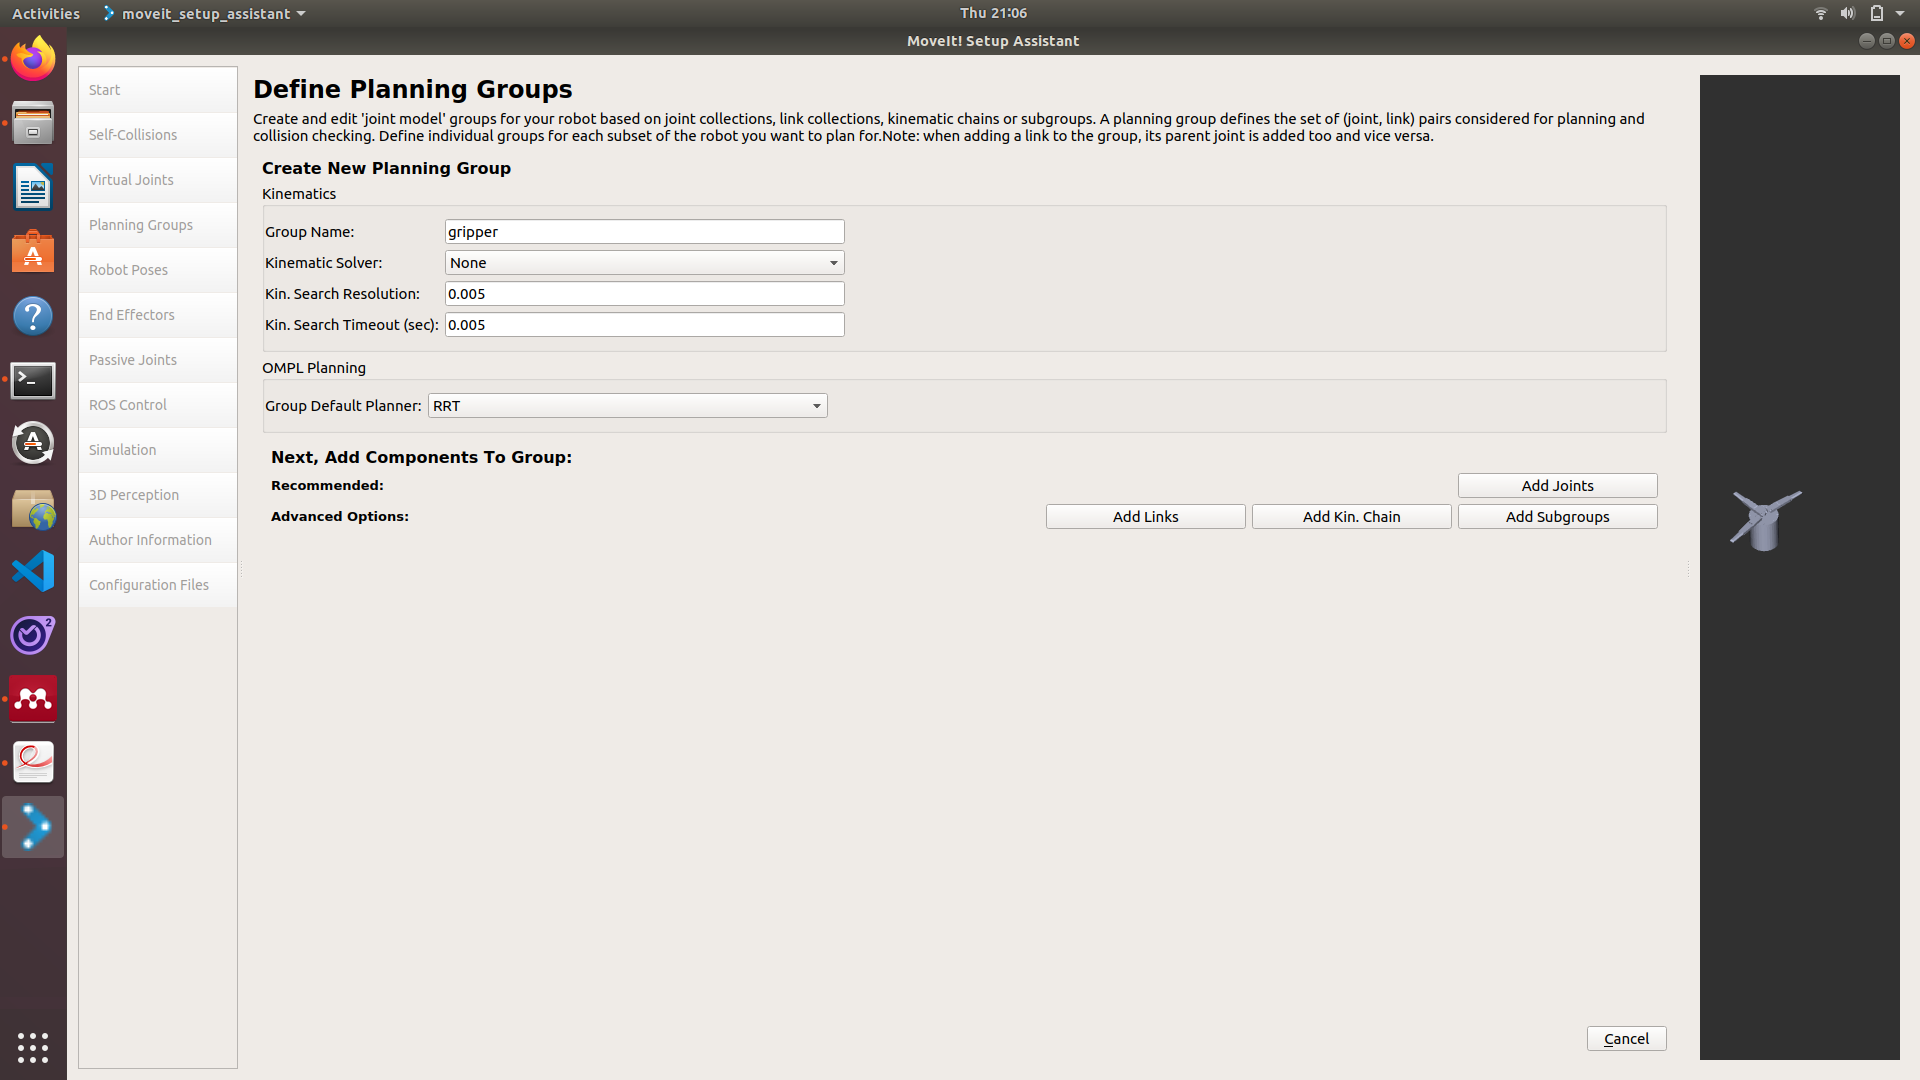
\includegraphics[scale=0.2]{gripper_images/planning_groups.png}
    \caption{Planning groups in MoveIt}
    \label{fig:my_label}
\end{figure}

\begin{figure}
    \centering
    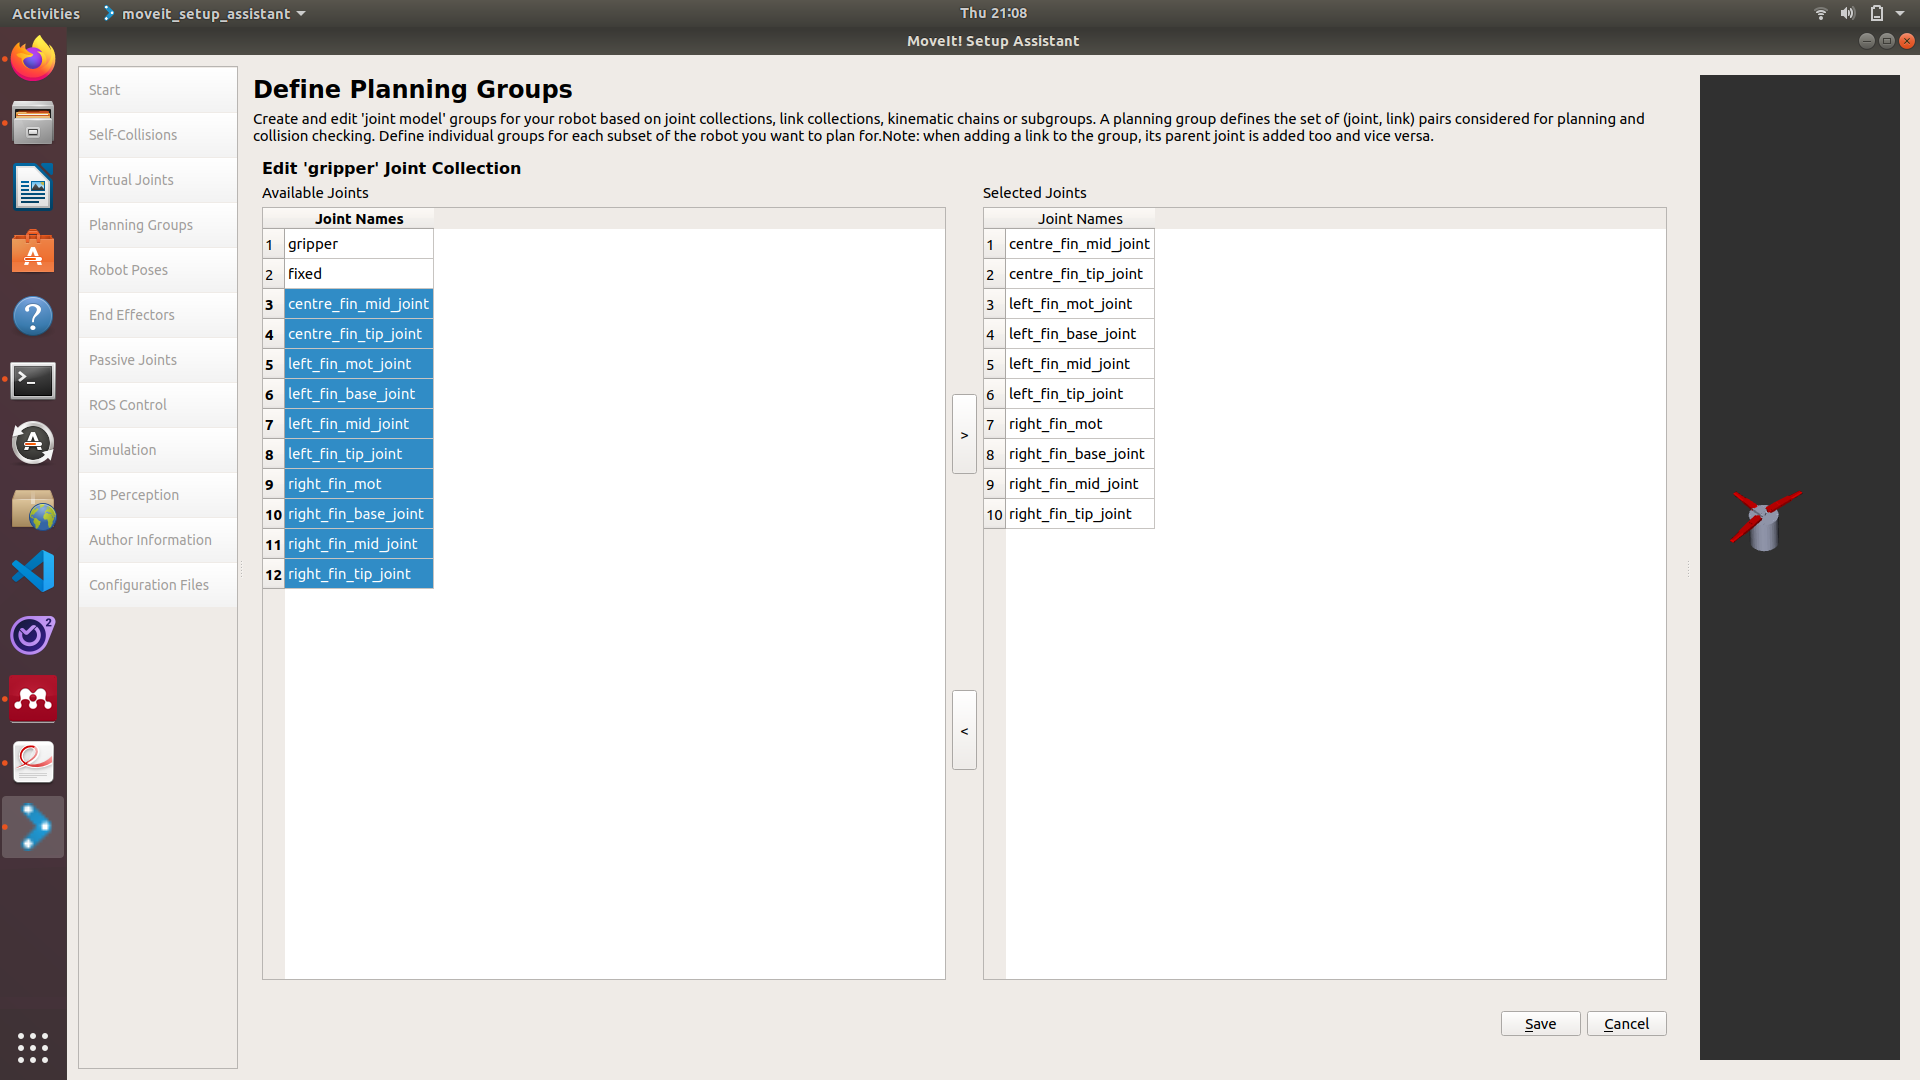
\includegraphics[scale=0.2]{gripper_images/planning_gp_joint.png}
    \caption{Defining Planning Groups}
    \label{fig:my_label}
\end{figure}





\item For adding different poses for robot, click on the \textbf{robot poses}
\item Next is adding \textbf{robot pose}, where fixed poses like the zero position and home position in the robot configuration are added.
\item The last step is to generate configuration files. Click on the \textbf{ Browse} button to locate a folder where  configuration file that is generated by the Setup Assistant tool has to be saved . 
\item After browsing the required folder, click on the \textbf{Generate Package} button, this will save the files into the chosen folder.
\item Click on\textbf{ Exit Setup Assistant}, which will exit us from the tool. 
\end{itemize}


\section{Motion planning of gripper in RViz}
Gazebo is a multi-robot simulator for outdoor environments.
Like Stage, it is capable of simulating a population of robots, sensors and objects, but does so in a three-dimensional world. It generates both realistic sensor feedback and physically plausible interactions between objects (it includes an accurate simulation of rigid body physics).
By realistically simulating robots and environments code
designed to operate a physical robot can be executed on
an artificial version. Numerous researchers have also used
Gazebo to develop and run experiments solely in a simulated
environment. Controlled experimental setups can easily be
created in which subjects can interact with manipulators in
a realistic manner.
There is a big difference between RViz visualisation and
Gazebo simulation, the former one is used to display relative
position of links, but the latter one can be regarded as an
experimental copy of real robot in virtual world.
\begin{itemize}
    \item \textbf{RViz} allows to create new planning scenes where robot works, generate motion plans, add new objects, visualize the planning output and can directly interact with the visualized robot. 
    MoveIt! package includes configuration files and launch files to start motion planning in RViz.
    \item Next step is visualization of the robot for that demo launch file is launched the command is \textbf{roslaunch gripper\_ demo.launch}.
    \item \textbf{RViz} window is opened which cosists of several tabs, on \textbf{context} tab from \textbf{OMPL} drop down list select \textbf{RRT}.
    \item Next is  \textbf{Planning} tab where, the start state, goal state plan a path, and execute the path of the robot can be assigned. 
    \end{itemize}
    \begin{figure}[!h]
    \centering
    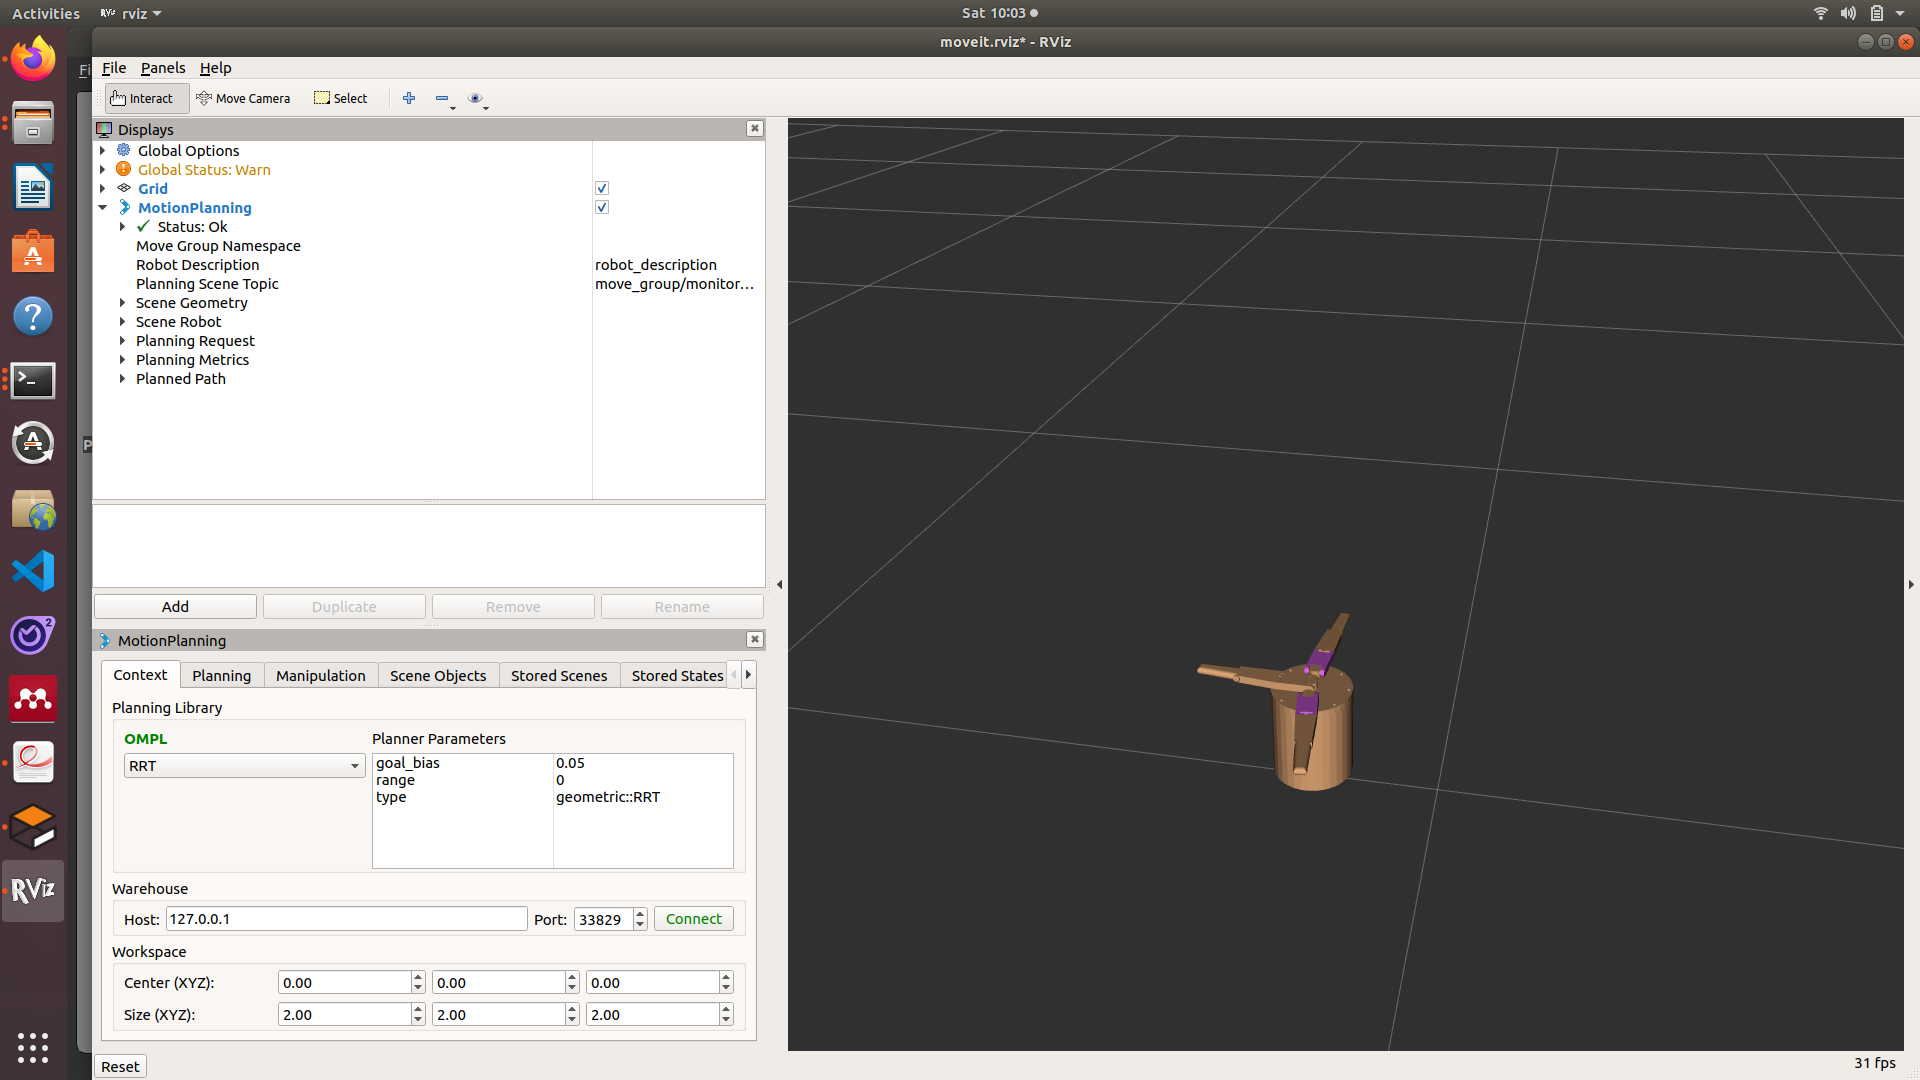
\includegraphics[scale=0.2]{gripper_images/planning_in_RViz.png}
    \caption{Motion planning of robot in RViz}
    \label{moveit_start}
    \end{figure}
    \textbf{Plan button}, is used to plan the path from the start to the goal state, and if the planning is successful, path can be executed by using 
    \textbf{Plan and Execute} button.

\section{ Gripper simulation using Gazebo}
\begin{itemize}
\item Gazebo is a multirobot simulator for complex indoor and outdoor robotic simulation. We can simulate complex robots, robot sensors, and a variety of 3D objects.
    \item The simulation model for the gripper by updating the existing robot description can be created by adding simulation parameters. 
    \item To launch the existing simulation model,  add \textbf{world.launch} and  \textbf{bringup.launch} files needs to be added to moveit! package.
    \item Now open a new terminal to launch Gazebo using the code \textbf{roslaunch gripper\_moveit\_config gazebo.launch}.
    \item \textbf{RViz} is used to control the robot on Gazebo, which creates a robotic environment similar to the real world. 
    \item After Gazebo, use the move\_group command and then launch RViz using the moveit\_rviz.launch command. The motion path planned on the RViz can now be achieved on  Gazebo.
    \item When the actual robot is fabricated, Gazebo is replaced by the robot and the robot can be controlled by using Rviz.
\end{itemize}

\par After completing all the above steps the robot can achieve the desired poses and rest of the interfacing using arduino can be seen in the next chapter. 



\subsection{Simulation in Gazebo}


\begin{figure}[!h]
\centering
%\vspace{0.4in}
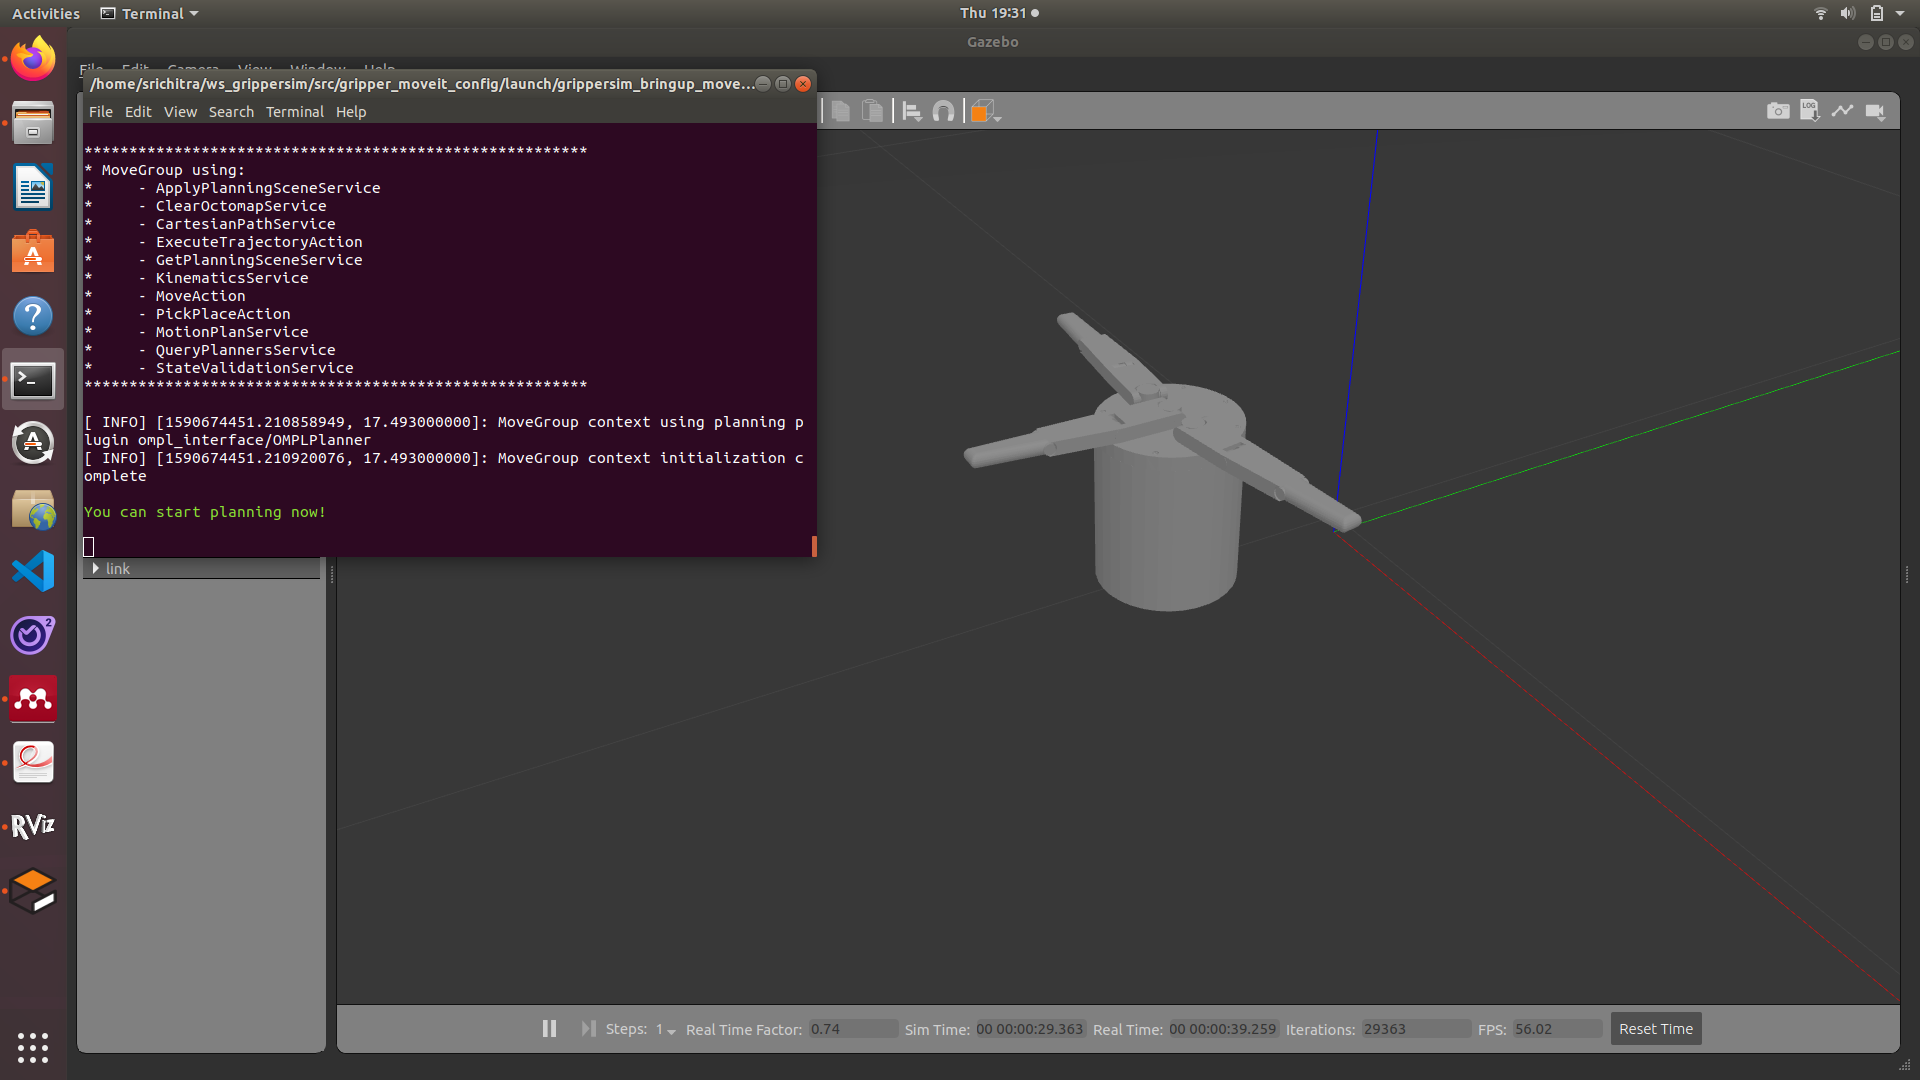
\includegraphics[scale=.2]{gripper_images/gripper_gazebo.png}
\caption{ Launching the model in Gazebo}
\label{joint_State}
\end{figure}


\begin{figure}[!h]
\centering
%\vspace{0.4in}
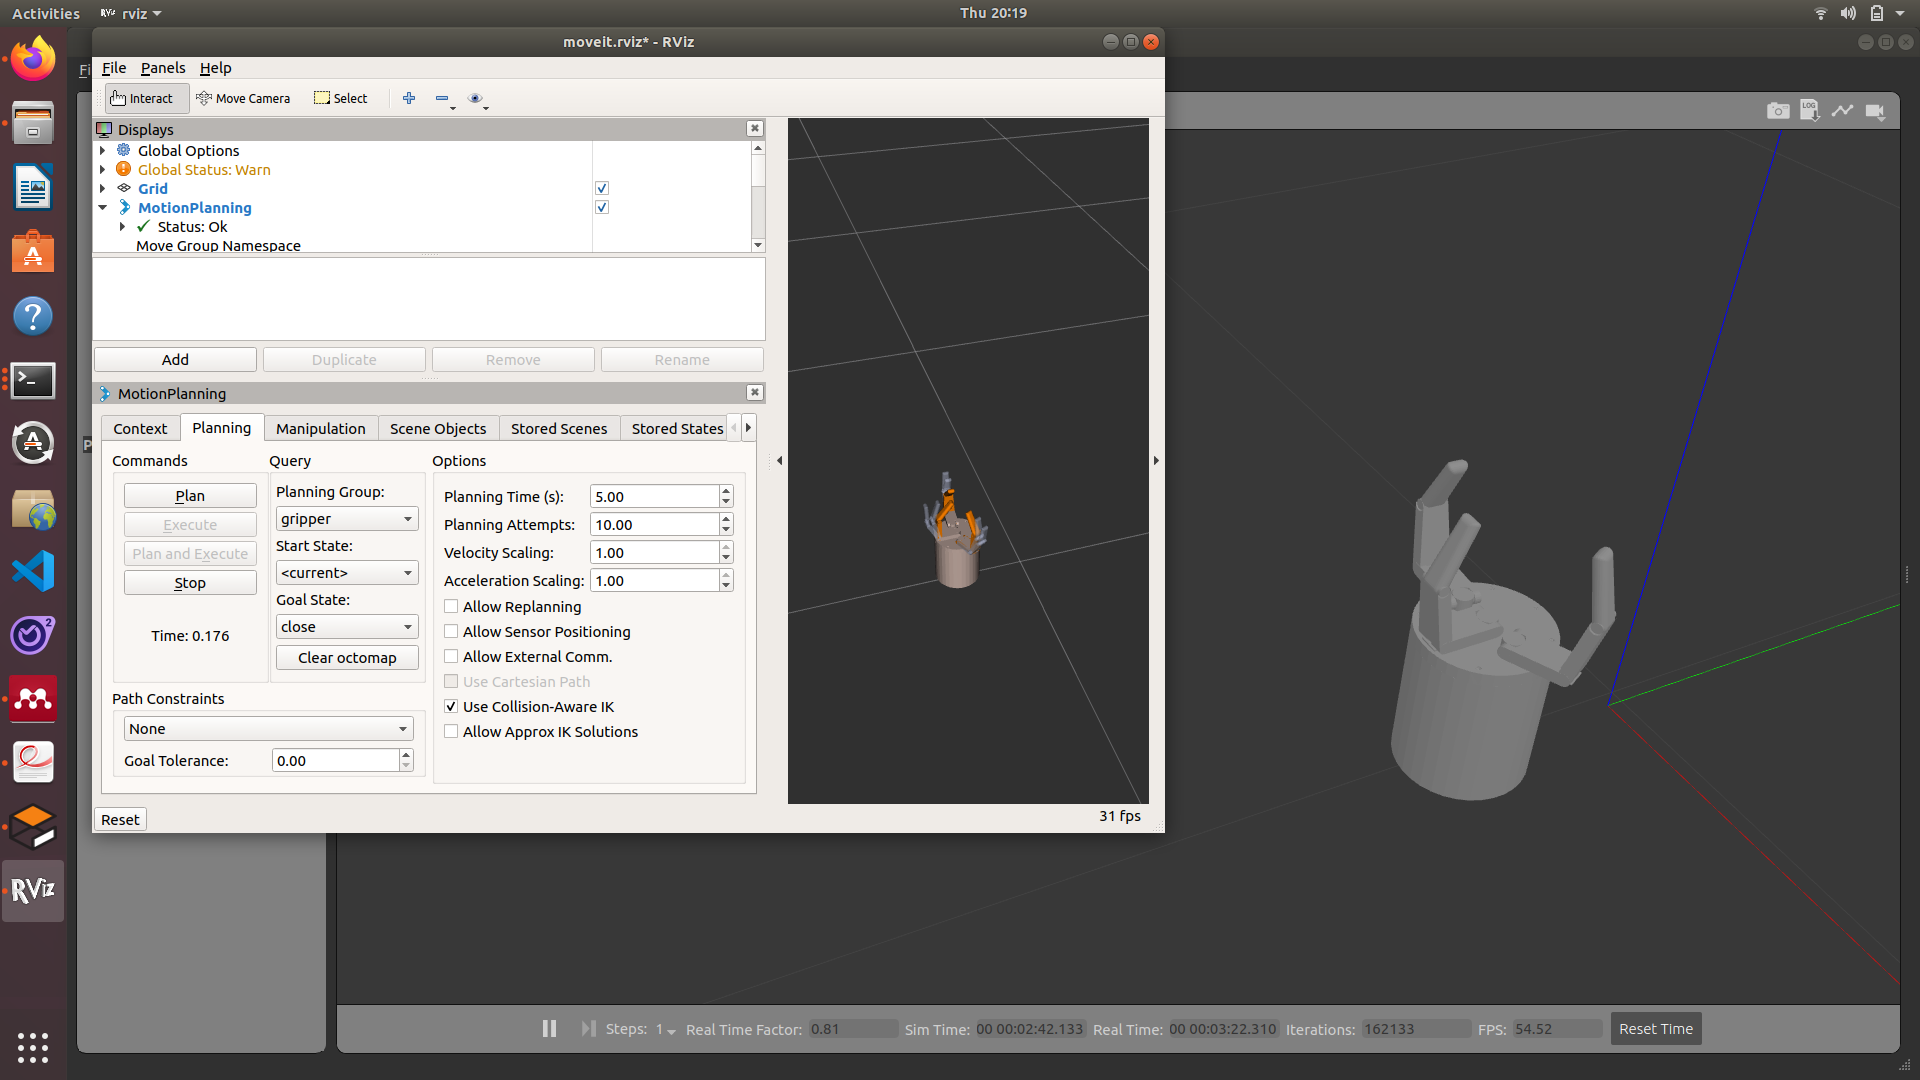
\includegraphics[scale=.2]{gripper_images/corresp_execution_in_gazebo.png}
\caption{Corresponding execution in Gazebo}
\label{joint_state_pub}
\end{figure}






%\chapter{Fabrication and Hardware Description} 




%\chapter{ROS Control Of Hardware}








\chapter{Simulation Results} 


\chapter{Conclusions} 


\chapter{References}



\end{document}